\documentclass[a4paper, 14pt]{extarticle}

% Поля
%--------------------------------------
\usepackage{geometry}
\geometry{a4paper,tmargin=2cm,bmargin=2cm,lmargin=3cm,rmargin=1cm}
%--------------------------------------


%Russian-specific packages
%--------------------------------------
\usepackage[T2A]{fontenc}
\usepackage[utf8]{inputenc} 
\usepackage[english, main=russian]{babel}
%--------------------------------------

\usepackage{textcomp}

% Красная строка
%--------------------------------------
\usepackage{indentfirst}               
%--------------------------------------             


%Graphics
%--------------------------------------
\usepackage{graphicx}
\graphicspath{ {../images/} }
\usepackage{wrapfig}
%--------------------------------------

% Полуторный интервал
%--------------------------------------
\linespread{1.3}                    
%--------------------------------------

%Выравнивание и переносы
%--------------------------------------
% Избавляемся от переполнений
\sloppy
% Запрещаем разрыв страницы после первой строки абзаца
\clubpenalty=10000
% Запрещаем разрыв страницы после последней строки абзаца
\widowpenalty=10000
%--------------------------------------

%Списки
\usepackage{enumitem}

%Подписи
\usepackage{caption} 

%Гиперссылки
\usepackage{hyperref}

\hypersetup {
	unicode=true
}

%Рисунки
%--------------------------------------
\DeclareCaptionLabelSeparator*{emdash}{~--- }
\captionsetup[figure]{labelsep=emdash,font=onehalfspacing,position=bottom}
%--------------------------------------

% \usepackage{tempora}

%Листинги
%--------------------------------------
\usepackage{listings}
\lstset{
  basicstyle=\ttfamily\footnotesize, 
  %basicstyle=\footnotesize\AnkaCoder,        % the size of the fonts that are used for the code
  breakatwhitespace=false,         % sets if automatic breaks shoulbd only happen at whitespace
  breaklines=true,                 % sets automatic line breaking
  captionpos=t,                    % sets the caption-position to bottom
  inputencoding=utf8,
  frame=single,                    % adds a frame around the code
  keepspaces=true,                 % keeps spaces in text, useful for keeping indentation of code (possibly needs columns=flexible)
  keywordstyle=\bf,       % keyword style
  numbers=left,                    % where to put the line-numbers; possible values are (none, left, right)
  numbersep=5pt,                   % how far the line-numbers are from the code
  xleftmargin=25pt,
  xrightmargin=25pt,
  showspaces=false,                % show spaces everywhere adding particular underscores; it overrides 'showstringspaces'
  showstringspaces=false,          % underline spaces within strings only
  showtabs=false,                  % show tabs within strings adding particular underscores
  stepnumber=1,                    % the step between two line-numbers. If it's 1, each line will be numbered
  tabsize=2,                       % sets default tabsize to 8 spaces
  title=\lstname                   % show the filename of files included with \lstinputlisting; also try caption instead of title
}
%--------------------------------------

%%% Математические пакеты %%%
%--------------------------------------
\usepackage{amsthm,amsfonts,amsmath,amssymb,amscd}  % Математические дополнения от AMS
\usepackage{mathtools}                              % Добавляет окружение multlined
\usepackage[perpage]{footmisc}
%--------------------------------------

%--------------------------------------
%			НАЧАЛО ДОКУМЕНТА
%--------------------------------------

\begin{document}

%--------------------------------------
%			ТИТУЛЬНЫЙ ЛИСТ
%--------------------------------------
\begin{titlepage}
    \thispagestyle{empty}
    \newpage


    %Шапка титульного листа
    %--------------------------------------
    \vspace*{-60pt}
    \hspace{-65pt}
    \begin{minipage}{0.3\textwidth}
        \hspace*{-20pt}\centering
        \includegraphics[width=\textwidth]{emblem}
    \end{minipage}
    \begin{minipage}{0.67\textwidth}\small \textbf{
            \vspace*{-0.7ex}
            \hspace*{-6pt}\centerline{Министерство науки и высшего образования Российской Федерации}
            \vspace*{-0.7ex}
            \centerline{Федеральное государственное бюджетное образовательное учреждение }
            \vspace*{-0.7ex}
            \centerline{высшего образования}
            \vspace*{-0.7ex}
            \centerline{<<Московский государственный технический университет}
            \vspace*{-0.7ex}
            \centerline{имени Н.Э. Баумана}
            \vspace*{-0.7ex}
            \centerline{(национальный исследовательский университет)>>}
            \vspace*{-0.7ex}
            \centerline{(МГТУ им. Н.Э. Баумана)}}
    \end{minipage}
    %--------------------------------------

    %Полосы
    %--------------------------------------
    \vspace{-25pt}
    \hspace{-35pt}\rule{\textwidth}{2.3pt}

    \vspace*{-20.3pt}
    \hspace{-35pt}\rule{\textwidth}{0.4pt}
    %--------------------------------------

    \vspace{1.5ex}
    \hspace{-35pt} \noindent \small ФАКУЛЬТЕТ\hspace{80pt} <<Информатика и системы управления>>

    \vspace*{-16pt}
    \hspace{47pt}\rule{0.83\textwidth}{0.4pt}

    \vspace{0.5ex}
    \hspace{-35pt} \noindent \small КАФЕДРА\hspace{50pt} <<Теоретическая информатика и компьютерные технологии>>

    \vspace*{-16pt}
    \hspace{30pt}\rule{0.866\textwidth}{0.4pt}

    \vspace{11em}

    \begin{center}
        \Large {\bf Лабораторная работа № 2} \\
        \large {\bf по курсу <<Языки и методы программирования>>} \\
        \large <<Разработка простейшего класса на языке Java>>
    \end{center}\normalsize

    \vspace{8em}


    \begin{flushright}
        {Студент группы ИУ9-22Б Бойко Р. А. \hspace*{15pt}\\
            \vspace{2ex}
            Преподаватель Посевин Д. П.\hspace*{15pt}}
    \end{flushright}

    \bigskip

    \vfill


    \begin{center}
        \textsl{Москва 2024}
    \end{center}
\end{titlepage}
%--------------------------------------
%		КОНЕЦ ТИТУЛЬНОГО ЛИСТА
%--------------------------------------

\renewcommand{\ttdefault}{pcr}

\setlength{\tabcolsep}{3pt}
\newpage
\setcounter{page}{2}

\section{Задание}\label{Sect::task}

Реализовать класс, представляющий неизменяемый многоугольник на плоскости, 
заданный координатами вершин, с двумя операциями: сдвиг многоугольника на заданное расстояние; 
поворот многоугольника вокруг указанной точки на заданный угол.
(Обе операции порожда􏰀т новые объекты.)


\section{Результаты}\label{Sect::res}

Исходный код программы представлен в листингах~\ref{lst:code1}--~\ref{lst:code3}.

\begin{lstlisting}[language={},caption={класс Point},label={lst:code1}]
public class Point {
    private double x, y;

    public Point(double x, double y) {
        this.x = x;
        this.y = y;
    }

    public double getX() {
        return x;
    }

    public void setX(double x) {
        this.x = x;
    }

    public double getY() {
        return y;
    }

    public void setY(double y) {
        this.y = y;
    }

    public double distanceTo(Point other) {
        double dx = this.x - other.getX();
        double dy = this.y - other.getY();
        return Math.sqrt(dx * dx + dy * dy);
    }

    public String toString() {
        return "(" + this.x + ", " + this.y + ")";
    }
}    
\end{lstlisting}

\begin{lstlisting}[language={},caption={класс ImmutablePolygon},label={lst:code2}]
import java.util.ArrayList;
import java.util.Collections;
import java.util.List;

public class ImmutablePolygon {
    private final List<Point> vertices;

    public ImmutablePolygon(List<Point> vertices) {
        this.vertices = Collections.unmodifiableList(new ArrayList<>(vertices));
    }

    public List<Point> getVertices() {
        return vertices;
    }

    public ImmutablePolygon shift(double deltaX, double deltaY) {
        List<Point> shiftedVertices = new ArrayList<>();
        for (Point vertex : vertices) {
            double newX = vertex.getX() + deltaX;
            double newY = vertex.getY() + deltaY;
            shiftedVertices.add(new Point(newX, newY));
        }
        return new ImmutablePolygon(shiftedVertices);
    }

    public ImmutablePolygon rotate(Point pivot, double angle) {
        List<Point> rotatedVertices = new ArrayList<>();
        double cosTheta = Math.cos(angle);
        double sinTheta = Math.sin(angle);
        for (Point vertex : vertices) {
            double dx = vertex.getX() - pivot.getX();
            double dy = vertex.getY() - pivot.getY();
            double newX = pivot.getX() + (dx * cosTheta - dy * sinTheta);
            double newY = pivot.getY() + (dx * sinTheta + dy * cosTheta);
            rotatedVertices.add(new Point(newX, newY));
        }
        return new ImmutablePolygon(rotatedVertices);
    }

    public String toString() {
        String result = "ImmutablePolygon{vertices=[";
        for (int i = 0; i < vertices.size(); i++) {
            result += vertices.get(i);
            if (i != vertices.size() - 1) {
                result += ", ";
            }
        }
        result += "]}";
        return result;
    }
}
\end{lstlisting}

\begin{lstlisting}[language={},caption={класс Test},label={lst:code3}]
import java.util.ArrayList;
import java.util.List;

public class Test {
    public static void main(String[] args) {

        // Создаем список координат вершин многоугольника
        List<Point> vertices = new ArrayList<>();
        vertices.add(new Point(0, 0));
        vertices.add(new Point(1, 0));
        vertices.add(new Point(1, 1));
        vertices.add(new Point(0, 1));

        // Создаем неизменяемый многоугольник
        ImmutablePolygon polygon = new ImmutablePolygon(vertices);

        // Выводим вершины многоугольника
        System.out.println("Original Polygon Vertices:");
        for (Point vertex : polygon.getVertices()) {
            System.out.println(vertex);
        }

        // Сдвигаем многоугольник на заданное расстояние
        ImmutablePolygon shiftedPolygon = polygon.shift(1, 1);
        System.out.println("\nShifted Polygon Vertices:");
        for (Point vertex : shiftedPolygon.getVertices()) {
            System.out.println(vertex);
        }

        // Поворачиваем многоугольник вокруг указанной точки на заданный угол
        Point pivot = new Point(0.5, 0.5);
        double angle = Math.PI / 2; // Поворот на 90 градусов (в радианах)
        ImmutablePolygon rotatedPolygon = polygon.rotate(pivot, angle);
        System.out.println("\nRotated Polygon Vertices:");
        for (Point vertex : rotatedPolygon.getVertices()) {
            System.out.println(vertex);
        }
    }
} 
\end{lstlisting}

Результат запуска представлен на рисунке~\ref{fig:lab2}.

\begin{figure}[!htb]
    \centering
    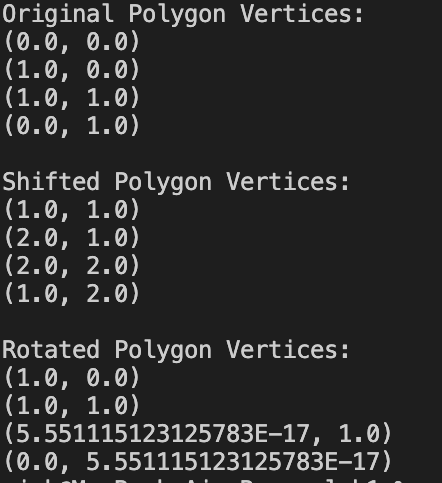
\includegraphics[width=0.8\textwidth]{lab2}
    \caption{Результат}
    \label{fig:lab2}
\end{figure}

\end{document}
